% flashcards-title: Two treatments of the same five plotted points
% flashcards-desc: Two small graphs side by side labeled P and Q, each showing the same five dots rising from lower left to upper right with small vertical wobbles. In P the dots are joined point to point by straight segments that bend at every dot. In Q a single straight line passes through the middle of the dots, some dots sitting slightly above the line and some slightly below it.
\documentclass[dvisvgm,tikz,border=8pt]{standalone}
\usepackage{tikz}
\usetikzlibrary{arrows.meta,calc,positioning}
\definecolor{DeckInk}{HTML}{172A3A}
\definecolor{DeckAccent}{HTML}{176B87}
\definecolor{DeckWarm}{HTML}{D97706}
\definecolor{DeckMuted}{HTML}{667784}
\definecolor{DeckPaper}{HTML}{F7FAFC}
\tikzset{
  every node/.style={font=\sffamily, text=DeckInk},
  object/.style={draw=DeckInk, line width=1.1pt, fill=DeckPaper},
  primary/.style={draw=DeckAccent, line width=1.5pt},
  boundary/.style={draw=DeckAccent, line width=1.5pt, dashed, rounded corners=6pt},
  guide/.style={draw=DeckMuted, line width=0.9pt, dashed},
  dimension/.style={{Stealth[length=3.2mm,width=2.2mm]}-{Stealth[length=3.2mm,width=2.2mm]}, draw=DeckWarm, line width=1.2pt},
  motion/.style={-{Stealth[length=3.5mm,width=2.5mm]}, draw=DeckAccent, line width=1.5pt, dashed},
}

\begin{document}
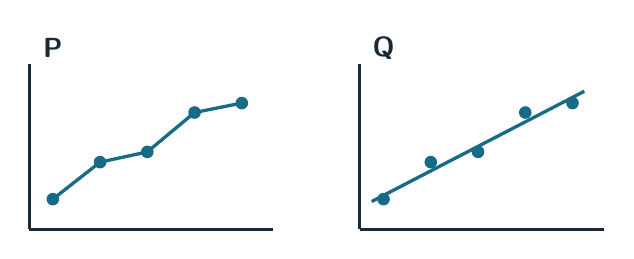
\begin{tikzpicture}[x=1cm,y=1cm]
  % Panel P
  \draw[DeckInk, line width=1.1pt] (0,0) -- (3.1,0);
  \draw[DeckInk, line width=1.1pt] (0,0) -- (0,2.1);
  \node[font=\sffamily\bfseries] at (0.3,2.3) {P};
  \draw[DeckAccent, line width=1.2pt] (0.3,0.38) -- (0.9,0.85) -- (1.5,0.98) -- (2.1,1.48) -- (2.7,1.60);
  \foreach \p in {(0.3,0.38),(0.9,0.85),(1.5,0.98),(2.1,1.48),(2.7,1.60)}
    \fill[DeckAccent] \p circle (0.08);
  % Panel Q
  \begin{scope}[xshift=4.2cm]
    \draw[DeckInk, line width=1.1pt] (0,0) -- (3.1,0);
    \draw[DeckInk, line width=1.1pt] (0,0) -- (0,2.1);
    \node[font=\sffamily\bfseries] at (0.3,2.3) {Q};
    \draw[DeckAccent, line width=1.2pt] (0.15,0.35) -- (2.85,1.75);
    \foreach \p in {(0.3,0.38),(0.9,0.85),(1.5,0.98),(2.1,1.48),(2.7,1.60)}
      \fill[DeckAccent] \p circle (0.08);
  \end{scope}
\end{tikzpicture}
\end{document}
